\documentclass[12pt,a4paper]{report}

%% ── Geometry and spacing ─────────────────────────────────────────────────
\usepackage[top=1in,bottom=1in,left=1.25in,right=1in]{geometry}
\usepackage{setspace}
\usepackage{emptypage}          % suppress headers on blank pages

%% ── Fonts and encoding ───────────────────────────────────────────────────
\usepackage[utf8]{inputenc}
\usepackage[T1]{fontenc}

%% ── Chapter / section formatting ─────────────────────────────────────────
\usepackage{titlesec}
\titleformat{\chapter}[block]{\Large\bfseries}{\thechapter.}{1em}{}
\titleformat{\section}[block]{\large\bfseries}{\thesection}{1em}{}
\titleformat{\subsection}[block]{\normalsize\bfseries}{\thesubsection}{1em}{}
\titleformat{\subsubsection}[block]{\normalsize\itshape}{\thesubsubsection}{1em}{}
\titlespacing*{\chapter}{0pt}{20pt}{15pt}

%% ── Header / footer ──────────────────────────────────────────────────────
\usepackage{fancyhdr}
\pagestyle{fancy}
\fancyhf{}
\fancyhead[L]{\small\leftmark}
\fancyhead[R]{\small\thepage}
\renewcommand{\headrulewidth}{0.4pt}
\fancypagestyle{plain}{\fancyhf{}\renewcommand{\headrulewidth}{0pt}}

%% ── Mathematics ──────────────────────────────────────────────────────────
\usepackage{amsmath,amssymb,amsfonts,amsthm}
\allowdisplaybreaks

%% ── Theorem-like environments ────────────────────────────────────────────
\newtheorem{theorem}{Theorem}[chapter]
\newtheorem{lemma}[theorem]{Lemma}
\newtheorem{proposition}[theorem]{Proposition}
\newtheorem{definition}{Definition}[chapter]
\newtheorem{remark}{Remark}[chapter]

%% ── Graphics and tables ──────────────────────────────────────────────────
\usepackage{graphicx}
\usepackage{subcaption}
\usepackage{float}
\usepackage{booktabs}
\usepackage{multirow}
\usepackage{tabularx}
\usepackage{rotating}
\usepackage{longtable}
\usepackage[labelfont=bf,font=small]{caption}
\graphicspath{{./plots/}{./}}

%% ── Lists ────────────────────────────────────────────────────────────────
\usepackage{enumitem}

%% ── Colour and hyperlinks ────────────────────────────────────────────────
\usepackage{xcolor}
\usepackage[hidelinks,
            colorlinks=true,
            linkcolor=black,
            citecolor=black,
            urlcolor=blue]{hyperref}

%% ── References ───────────────────────────────────────────────────────────
\usepackage[numbers,sort&compress]{natbib}
\bibliographystyle{plainnat}

%% ── Algorithm ────────────────────────────────────────────────────────────
\usepackage{algorithm}
\usepackage{algpseudocode}

%% ── URL ──────────────────────────────────────────────────────────────────
\usepackage{url}

%% ── Math operators and shortcuts ─────────────────────────────────────────
\DeclareMathOperator{\Cov}{Cov}
\DeclareMathOperator{\Var}{Var}
\newcommand{\bZ}{\mathbf{Z}}
\newcommand{\bz}{\mathbf{z}}

%% ── Appendix ─────────────────────────────────────────────────────────────
\usepackage[title,titletoc]{appendix}

%% =========================================================================
\begin{document}
\onehalfspacing
%% =========================================================================

%% ── Title Page ───────────────────────────────────────────────────────────
\thispagestyle{empty}
\begin{center}
    {\Large\textbf{Indian Institute of Technology Delhi}}\\[0.3cm]
    {\large Department of Mathematics}\\[2cm]

    \includegraphics[width=0.28\textwidth]{iitd_logo.jpg}\\[1.5cm]

    {\Large\textbf{M.Tech. Project Final Report}}\\[1.2cm]

    {\LARGE\textbf{Causal Learning for Strategic Policy Design\\[0.3cm]
    (Based on NFHS-5)}}\\[2cm]

    \textbf{Submitted by:}\\[0.3cm]
    {\large Abdhesh Dash}\\[0.2cm]
    Roll No.:\ 2021MT60945\\[1.0cm]

    \textbf{Supervisor:}\ Prof.\ Rahul Singh\\[0.2cm]
    \textbf{Co-Supervisor:}\ Prof.\ Biplab Paul\\[0.2cm]
    Department of Mathematics\\
    Indian Institute of Technology Delhi\\[2cm]

    June 2026
\end{center}
\newpage

%% ── Declaration ──────────────────────────────────────────────────────────
\thispagestyle{empty}
\chapter*{Declaration}
I certify that the work contained in this report has been carried out by me
under the guidance of Prof.\ Rahul Singh and Prof.\ Biplab Paul,
Department of Mathematics, Indian Institute of Technology Delhi.
This work has not been submitted for the award of any other degree or
diploma.

\vspace{3cm}
\noindent
\begin{tabular}{ll}
\textbf{Abdhesh Dash} & \hspace{6cm} \textbf{Prof.\ Rahul Singh}\\[0.3cm]
2021MT60945             & \hspace{6cm} (Supervisor)\\[2.5cm]
Date:                & \hspace{6cm} \textbf{Prof.\ Biplab Paul}\\[0.3cm]
                      & \hspace{6cm} (Co-Supervisor)
\end{tabular}
\newpage

%% ── Abstract ─────────────────────────────────────────────────────────────
\chapter*{Abstract}
\addcontentsline{toc}{chapter}{Abstract}

Population health policy in low- and middle-income countries requires moving
beyond association to causation: identifying which modifiable indicators, when
improved, produce the largest gains in health outcomes.
We present a data-driven causal learning framework applied to the fifth round
of India's National Family Health Survey (NFHS-5), covering 131 standardised
indicators across all 36 states and union territories.

The pipeline proceeds in four stages: (i)~hierarchical clustering of 131
indicators into 32 thematically coherent groups using merge-height and
within-cluster cohesion diagnostics; (ii)~two-level PC-algorithm causal
discovery (intra-cluster and inter-cluster meta-variable DAGs) with 100-resample
bootstrap edge-confidence filtering; (iii)~a three-criterion screening procedure
(directional asymmetry $\Delta\ge0.10$, undirected-edge fraction $\beta<0.30$,
partial-correlation residual $|\rho|\ge0.35$) with empirically calibrated
thresholds; and (iv)~Average Treatment Effect (ATE) estimation along six
validated pathways using four complementary estimators (IPW, DR Learner,
T-Learner, X-Learner), with cross-estimator sign consistency as the primary
evidence criterion.

All six pathways achieve pooled consistency: Family Planning (Any) reduces
unmet spacing need ($-3.22$\,pp), raises neonatal tetanus protection
($+5.55$\,pp), and is linked to a C-section pathway via elevated blood pressure
($+9.71$\,pp); first-trimester ANC raises facility-seeking for home births
($+1.70$\,pp); women's literacy increases mobile phone ownership ($+14.94$\,pp);
and men's internet use is causally associated with men's literacy ($+4.47$\,pp).
Stratified analysis reveals systematic effect heterogeneity: literacy effects on
mobile ownership are nearly twice as large in rural settings and increase
monotonically with income, indicating a demand-pull mechanism.
These findings demonstrate that area- and income-stratified causal estimation
should be the analytical default for NFHS-based policy design.

\vspace{1em}
\noindent\textbf{Keywords:} Causal inference, NFHS-5, Public health policy,
India, PC algorithm, Average Treatment Effect, Graph clustering, Stratified
analysis, Causal structure learning, Machine learning, Doubly Robust estimation.

\newpage

%% ── Table of Contents, Figures, Tables ──────────────────────────────────
\tableofcontents
\newpage
\listoffigures
% \newpage
\listoftables
\newpage

%% =========================================================================
\chapter{Introduction}
\label{chap:intro}
%% =========================================================================

Population health in low- and middle-income countries is shaped by a dense web of
socioeconomic, behavioural, and biological processes that interact in non-obvious
ways.
Policy interventions like investments in sanitation, family-planning programmes,
nutrition campaigns are costly and politically constrained, so their expected
effects must be estimated rigorously before deployment.
Standard approaches in public health rely on observational associations drawn from
large-scale surveys, yet association does not imply causation.
A positive correlation between maternal literacy and child vaccination uptake may
reflect a shared confounder (household wealth) rather than a direct effect of
education; acting on spurious correlations wastes resources and may cause harm
\citep{pearl2009causality,hernan2020causal}.

Causal inference provides a principled framework for moving beyond association.
Rather than asking \emph{which indicators co-move}, it asks \emph{what would happen
if we intervened on a specific indicator}---a question that maps directly onto policy
design.
Prior work has applied causal methods to maternal and child health data:
instrumental variable designs have estimated the effect of institutional delivery
on neonatal mortality \citep{Lim2010}, propensity-score methods have examined
skilled-birth attendance \citep{Bhutta2008}, and doubly-robust estimators have been
deployed on Demographic and Health Survey data to study anaemia and stunting
\citep{Luque2019,Kennedy2020}.
However, most such analyses treat indicator pairs in isolation, ignoring the
multi-dimensional dependency structure that governs how exposures and outcomes
co-evolve across a national health system.

The empirical foundation of this study is the fifth round of India's National Family
Health Survey (NFHS-5), conducted during 2019--2021 \citep{nfhs5report}, covering
131 standardised indicators (health, nutrition, family planning, women empowerment,
education, etc.) across all 36 states and union territories.
The resulting dataset is a high-dimensional observational system in which
socioeconomic context, health behaviours, and biological outcomes are jointly
recorded.

Our framework proceeds in four stages.
\emph{Structure discovery}: a correlation architecture is recovered, indicators are
grouped into thematically coherent clusters via hierarchical clustering, and a
two-level PC algorithm \citep{spirtes2000causation} with bootstrap validation
identifies candidate directed pathways.
\emph{Causal screening}: three empirically calibrated criteria separate causal edges
from confounding artefacts.
\emph{Causal effect estimation}: for each of six validated pathways, the ATE is
estimated via four complementary estimators.
\emph{Heterogeneity analysis}: estimation is stratified by rural/urban area type
and per-capita GSDP tertile.

\section{Contributions}

Our contributions are as follows:
\begin{enumerate}[leftmargin=*,itemsep=4pt]
\item We propose a scalable observational causal analysis pipeline combining
  graph-based indicator clustering with two-level constraint-based causal discovery,
  making PC-algorithm structure learning tractable on a 131-indicator national health
  survey.
\item We calibrate a principled three-criterion causal screening procedure
  (directional asymmetry, undirected-edge fraction, partial-correlation residual)
  using KDE trough, Jenks natural break, and F1-proxy analysis, providing
  data-justified thresholds rather than arbitrary cut-points.
\item We evaluate four complementary causal ML estimators (IPW, DR Learner,
  T-Learner, X-Learner) across six directed pathways inferred from NFHS-5,
  reporting 95\% bootstrap confidence intervals and cross-estimator sign consistency.
\item We demonstrate that area- and income-stratified estimation substantially
  changes causal conclusions relative to pooled inference, and justify this choice
  via CATE heterogeneity analysis.
\item We provide a transparent five-stage pathway selection procedure from 88
  bootstrap-screened edges to 6 final pathways, eliminating domain-implausible
  relationships.
\end{enumerate}

\section{Organisation of the Report}

Chapter~\ref{chap:related} reviews related work.
Chapter~\ref{chap:data} describes the dataset and preprocessing.
Chapter~\ref{chap:framework} formalises the causal inference framework.
Chapter~\ref{chap:clustering} presents the graph clustering methodology.
Chapter~\ref{chap:ate} describes the ATE estimation pipeline.
Chapter~\ref{chap:results} reports experimental results.
Chapters~\ref{chap:discussion} and \ref{chap:conclusion} discuss findings and
conclude. Appendices contain proofs, supplementary tables, and figures.

%% =========================================================================
\chapter{Related Work}
\label{chap:related}
%% =========================================================================

\section{Causal Inference in Population Health}

Causal methods have been applied to health survey data with growing frequency.
\citet{Lim2010} used instrumental variables to estimate the effect of institutional
delivery on neonatal mortality in South Asia.
\citet{Bhutta2008} applied propensity-score matching to skilled-birth attendance.
Doubly-robust methods were used by \citet{Luque2019} and \citet{Kennedy2020} on DHS
data to study anaemia and stunting.

Constraint-based causal discovery algorithms, particularly the PC algorithm
\citep{spirtes2000causation}, have been applied to biomedical data to recover
directed acyclic graphs from observational data under the faithfulness and Markov
assumptions.
\citet{kalisch2007estimating} showed that PC scales to high-dimensional settings
using $\ell_1$-penalised conditional independence tests.
Bootstrap aggregation over PC outputs to quantify edge stability was formalised by
\citet{friedman1999learning}.

Machine learning-augmented causal estimators have expanded estimation accuracy in
small and moderate samples.
The doubly robust DR Learner \citep{chernozhukov2018doubleml} achieves
$\sqrt{n}$-consistency if either the propensity or outcome model is correct.
Meta-learner frameworks (T-Learner, X-Learner) were systematically compared by
\citet{kunzel2019metalearners}, who showed that the X-Learner's
propensity-weighted imputation reduces variance under treatment group imbalance.
\citet{nie2021quasioracle} showed that the R-Learner achieves minimax optimality
on CATE estimation; the DR Learner is a special case.
DoWhy \citep{sharma2020dowhy}, EconML \citep{econml}, and CausalML
\citep{chen2020causalml} provide production-grade implementations.

CATE heterogeneity analysis provides direct empirical justification for stratified
estimation \citep{wager2018estimation,athey2016recursive}.
When CATE distributions differ between rural and urban strata, pooled ATE is a
weighted average of signals that may even oppose in sign, a form of Simpson's
paradox \citep{pearl2009causality}.

\section{NFHS and Indian Health Policy Analysis}

The NFHS series is the principal source for population health statistics in India
\citep{nfhs5report}.
Previous NFHS-based studies have examined women's empowerment \citep{vignitha2024women}
and contraceptive uptake \citep{sedgh2016unmet}, but typically treat indicator pairs
in isolation without a formal causal framework.
Economic development has been identified as a structural confounder in cross-state
Indian health analyses \citep{thorn1968per,hordofa2023moderating}.
The mismatch between economic ranking and health outcomes in Indian states
\citep{viswanathan2021growth} illustrates why causal rather than correlational
analysis is essential.

\section{Graph-Based Indicator Clustering}

Community detection algorithms have been applied to correlation networks in
economics and epidemiology.
Louvain \citep{blondel2008fast} and Leiden \citep{traag2019louvain} maximise
modularity on weighted graphs; spectral clustering via the graph Laplacian
\citep{ng2002spectral} provides a geometric alternative.
To the best of our knowledge, no prior work has systematically swept and compared
all four clustering paradigms on a health indicator network and selected the best
partition for downstream causal PC search using a combined Silhouette--Modularity--NMI
ranking.

%% =========================================================================
\chapter{Dataset and Preprocessing}
\label{chap:data}
%% =========================================================================

\section{NFHS-5 Survey}

NFHS-5 was conducted during 2019--2021 \citep{nfhs5report} and covers 131
standardised indicators spanning fertility, nutrition, health behaviour, and social
determinants across all 28 states and 8 union territories.
The survey employed a stratified, two-stage sampling design with approximately
636,699 households interviewed, yielding data from 724,115 women aged 15--49 and
101,839 men aged 15--54.
NFHS-5 reports each indicator separately for \emph{Rural}, \emph{Urban}, and
\emph{Total} strata, enabling area-stratified causal analysis without approximation.

\section{Per-Capita GSDP Data}

State-level per-capita Gross State Domestic Product (GSDP) for the NFHS-5
reference period was obtained from the Open Government Data Platform India
\citep{ogd_gsdp_2023}.
States are assigned to income tertiles (\textit{Low}, $\lesssim$\,Rs.\,90k;
\textit{Moderate}; \textit{High}, $\gtrsim$\,Rs.\,180k per capita).
Three union territories with missing GSDP are excluded, leaving $n=33$ analysis
units.

\section{Preprocessing}

\begin{enumerate}[leftmargin=*,itemsep=4pt]
\item \textbf{Name standardisation.} Inconsistent state spellings are harmonised.
\item \textbf{Missing-value handling.} Suppressed cells (``*'') are recoded to
  \texttt{NaN}; all 131 indicators are coerced to numeric; rows with $>50\%$
  missing values are dropped.
\item \textbf{Column selection.} Administrative identifiers are excluded; the 131
  numeric indicator columns form the analytical feature set.
\item \textbf{Positivity check.} For each causal pathway, the complete-case subset
  must have $n\ge8$ states.
\end{enumerate}

Full details are in Appendix~\ref{app:data_construction}.

%% =========================================================================
\chapter{Causal Structure Learning Framework}
\label{chap:framework}
%% =========================================================================

\section{Structural Causal Models}

A structural causal model (SCM) encodes the data-generating mechanism as
\[
X_i := f_i(\mathrm{Pa}_i,\, U_i), \quad i = 1,\ldots,d,
\]
where $\mathrm{Pa}_i$ denotes the parents of $X_i$ in a directed acyclic graph
(DAG) and $U_i$ are mutually independent exogenous noise variables
\citep{pearl2009causality}.
For a health outcome $Y$, exposure $X$, and covariates $Z$ this specialises to
$Y = f_Y(X,Z,U_Y)$, $X = f_X(Z,U_X)$.

\section{Interventional Distributions and the Do-Operator}

Observational summaries describe $E[Y \mid X=x]$, while causal reasoning concerns
\[
E[Y \mid \mathrm{do}(X=x)],
\]
the expected outcome when $X$ is externally set to $x$, removing all incoming edges
to $X$ in the DAG \citep{pearl2009causality}.
Under the backdoor criterion (Appendix~\ref{app:defs}, Definition~\ref{def:backdoor}):
\[
P\!\left(Y \mid \mathrm{do}(X=x)\right) = \sum_z P(Y \mid X=x,Z=z)\,P(Z=z).
\]

\section{Average Treatment Effect}

Under consistency, conditional ignorability, and positivity
(Appendix~\ref{app:defs}), the ATE is identified as:
\begin{equation}
\mathrm{ATE}
= E[Y(1) - Y(0)]
= E_Z\!\bigl[E[Y \mid X=1,Z] - E[Y \mid X=0,Z]\bigr].
\label{eq:ate}
\end{equation}

\section{PC Algorithm for Causal Discovery}

The PC algorithm \citep{spirtes2000causation} recovers the DAG skeleton by
iteratively testing conditional independence $X_i \perp\!\!\!\perp X_j \mid S$,
removing edges when independence holds, then orienting remaining edges through
v-structure rules.
Because complexity scales as $O(n^k)$ in the number of variables $n$ and maximum
degree $k$ \citep{kalisch2007estimating}, applying PC directly to all 131 NFHS
indicators is computationally intractable, motivating the two-level architecture
described in Chapter~\ref{chap:ate}.

%% =========================================================================
\chapter{Graph Clustering Methodology}
\label{chap:clustering}
%% =========================================================================

\section{Correlation Distance and Rank Structure}

A correlation-distance matrix $D_{ij} = 1 - |\rho_{ij}|$ embeds indicators in a
similarity space.
Rank plots of pairwise correlations across overall, area-stratified,
income-stratified, and partial-correlation stratifications
(Appendix~\ref{app:corr}) reveal: (i)~right-skewed distributions with ${\sim}10$
pairs exceeding $|r|=0.70$; (ii)~rural correlations are stronger than urban at
every rank; (iii)~GSDP suppresses rather than inflates associations.

Preliminary mediation analysis (Appendix~\ref{app:mediation}) confirmed that
per-capita GSDP is a weak direct confounder (proportion mediated $=-2.14\%$);
women's literacy is the dominant mediating channel and is adopted alongside GSDP
as the joint confounder set $\bZ$.

\section{Hierarchical Clustering and Cluster-Count Selection}

Average-linkage agglomerative clustering minimises inter-cluster distance,
\[
d(A,B) = \frac{1}{|A||B|}\sum_{i\in A}\sum_{j\in B} D_{ij},
\]
producing dendrograms aligned with recognisable development domains \citep{murtagh2014ward}.
The number of clusters $k$ is selected via two evidence-based diagnostics
(Figure~\ref{fig:hier_cluster_selection}):
\begin{itemize}[itemsep=2pt]
\item \textbf{Merge-height elbow.} Large jumps between consecutive merge heights
  signal natural cut-points \citep{tibshirani2001estimating}.
\item \textbf{Within-cluster cohesion.} The elbow in
  $\bar{D}(k)$ marks diminishing returns \citep{thorndike1953belongs}.
\end{itemize}
Both diagnostics converge on $k\in[28,36]$; $k=32$ is chosen as the knee of the
cohesion curve with mean intra-cluster distance $\bar{D}<0.30$.

\begin{figure}[H]
\centering
\includegraphics[width=1.05\textwidth]{plots/hierarchical_n_clusters.png}
\caption{Hierarchical clustering diagnostics: (left) dendrogram merge heights,
  (centre) first-difference height gaps, (right) within-cluster cohesion curve.
  Red dashed line marks the chosen $k=32$.}
\label{fig:hier_cluster_selection}
\end{figure}

\section{Graph-Based Clustering}

Indicators form a weighted correlation network $G=(V,E,W)$ with
$w_{ij}=|\rho_{ij}|$.
Community detection maximises modularity \citep{blondel2008fast}:
\begin{equation}
Q = \frac{1}{2m}\sum_{ij}\!\left(A_{ij}-\frac{k_ik_j}{2m}\right)\delta(c_i,c_j).
\label{eq:modularity}
\end{equation}
Resolution sweeps over $\gamma\in\{0.5,\ldots,6.0\}$ select $\gamma=3.0$ for both
Louvain and Leiden (silhouette peak; aligned with hierarchical $k=32$).
Spectral clustering \citep{ng2002spectral} uses $k=28$ (local silhouette maximum
$=0.2016$).

\section{Clustering Method Selection}

Four candidate partitions are evaluated on Silhouette, Modularity $Q$, and mean
pairwise NMI \citep{strehl2002cluster} (Table~\ref{tab:clustering_eval}).
Each method is ranked on each metric; the combined rank (lower = better)
determines the method used for PC algorithm input.

\begin{table}[H]
\centering
\caption{Clustering evaluation. Combined rank (sum of per-metric ranks; lower is
  better) determines the method used as input to the PC algorithm.}
\label{tab:clustering_eval}
\renewcommand{\arraystretch}{1.3}
\begin{tabular}{lrrrr}
\toprule
\textbf{Method} & \textbf{Silhouette} & \textbf{Modularity} &
\textbf{Mean NMI} & \textbf{Combined rank} \\
\midrule
Hierarchical & \textbf{0.2541} & 0.3945 & 0.6968 & \textbf{4}  \\
Leiden       & 0.2096          & 0.3709 & \textbf{0.7273} & 5   \\
Spectral     & 0.2016          & 0.2586 & 0.6850 & 9            \\
Louvain      & $-$0.1660       & 0.0753 & 0.6070 & 12           \\
\bottomrule
\end{tabular}
\end{table}

Hierarchical clustering achieves the highest silhouette and lowest combined rank
and is selected for the PC algorithm.

\begin{figure}[H]
\centering
\includegraphics[width=0.55\textwidth]{plots/nmi_heat_map.png}
\caption{Pairwise NMI heatmap between four clustering solutions. High
  Leiden--Hierarchical ($0.780$) and Spectral--Hierarchical ($0.726$) NMI
  confirm consensus on the latent partition.}
\label{fig:nmi_heatmap}
\end{figure}

%% =========================================================================
\chapter{ATE Estimation Pipeline}
\label{chap:ate}
%% =========================================================================

\section{Two-Level Causal Discovery Architecture}
\label{sec:twolevel}

A two-level DAG architecture manages the $O(n^k)$ complexity of the PC algorithm
while preserving cross-domain causal relationships.
\textbf{Level 1 (intra-cluster):} the PC algorithm is applied within each of the
32 hierarchical clusters independently, recovering intra-domain directed edges.
\textbf{Level 2 (inter-cluster):} each cluster $C_k$ is summarised by a
meta-variable $Z_k = |C_k|^{-1}\sum_{X_i\in C_k}X_i$; the PC algorithm is then
applied on the 32 meta-variables to recover cross-domain directed pathways.

This decomposition is theoretically justified by the local Markov property of DAGs
\citep{chickering2002optimal,spirtes2000causation}:
if within-cluster indicators satisfy the cluster-level Markov condition, then the
inter-cluster meta-variable DAG captures the essential cross-domain causal
structure without running PC on all 131 indicators simultaneously.
Clustering reduces each PC run to at most $|$cluster$|\le6$ variables
($\binom{6}{2}=15$ pairs); the meta-variable run operates on only 32 nodes.

\section{Bootstrap Edge Screening and Three-Criterion Causal Filtering}

\subsection*{Bootstrap Aggregation}

The PC algorithm is applied over $B=100$ resamples (with replacement) of the
$n$ states; $\hat{P}(i\to j) = B^{-1}\sum_{b=1}^B\mathbf{1}\{i\to j\in G^{(b)}\}$
\citep{friedman1999learning}.
The 88 collected edge-direction pairs enter a three-stage filtering process.

\subsection*{Threshold Calibration}

The three screening thresholds were calibrated empirically using distributional
analysis (KDE and Jenks natural breaks \citep{jenks1967data}) and
sensitivity-based analyses (Appendix~\ref{app:threshold_calibration}).
The final values, $\Delta=0.10$, $\beta<0.30$, and $|\rho|\ge0.35$, correspond to
stable regions of the calibration curves and retain 43 of 88 candidate
edge-direction pairs.

\subsection*{Three-Criterion Causal Screening}

\begin{enumerate}[leftmargin=*,itemsep=4pt]
\item \textbf{Directional asymmetry $\ge0.10$:}
  $\alpha_{AB} = \hat{P}(A\to B)-\hat{P}(B\to A) \ge 0.10$.
  Edges with $|\alpha_{AB}|<0.10$ are orientation-ambiguous
  \citep{spirtes2000causation}.
\item \textbf{Undirected-edge fraction $<0.30$:}
  Edges appearing undirected in $\ge30\%$ of resamples lack sufficient orientation
  evidence.
\item \textbf{Partial-correlation residual $|\rho_{AB\cdot Z}|\ge0.35$:}
  After regressing out GSDP and women's literacy, the residual association must
  survive \citep{pearl2009causality}.
\end{enumerate}
Of 88 bootstrap edges, 43 pass all three criteria; 18 are further removed by the
domain-plausibility filter, leaving 25 final candidates.

\begin{figure}[H]
\centering
\includegraphics[width=0.72\textwidth]{plots/direction_asymm_distribution.png}
\caption{Direction-asymmetry distribution for all bootstrap edges. Blue: causal
  (passed all three criteria); red: rejected. Rejected edges concentrate near
  $\alpha\approx0.1$, consistent with bidirectional confounding.}
\label{fig:causal_screening}
\end{figure}

\section{Pathway Selection: From 88 Edges to 6 Final Pathways}
\label{sec:pathway_selection}

Six final pathways were obtained through five sequential stages:

\begin{description}[leftmargin=2em,itemsep=4pt]
\item[Stage 1 -- Bootstrap PC discovery.]
  The PC algorithm is run over $B=100$ resamples across all 32 clusters and the 32
  meta-variables. A total of 88 bootstrap edge-direction pairs are collected.

\item[Stage 2 -- Three-criterion screening.]
  Applying the empirically calibrated thresholds reduces the set from 88 to 43 edges.

\item[Stage 3 -- Domain-plausibility filtering.]
  Eighteen edges are removed: (i)~severity pairs, (ii)~gender mirrors,
  (iii)~temporally implausible directions, and (iv)~demographic count variables
  acting as purported causes of clinical outcomes. This leaves 25 candidates.

\item[Stage 4 -- Candidate pool of 14.]
  Fourteen pathways are retained as candidates after inspection over 4--5
  independent pipeline runs. The 14 candidates are listed in
  Appendix~\ref{app:pathway_selection}.

\item[Stage 5 -- Final 6 by estimator and stratification consistency.]
  The four-estimator ATE pipeline is applied to all 14 candidates.
  The six pathways reported here achieve: (a)~consistent sign agreement
  ($\ge3/4$ estimators) under pooled estimation; and (b)~consistent sign agreement
  under at least two of the three area strata and two of the three income strata.
\end{description}

\noindent The six final pathways are:
\begin{enumerate}[leftmargin=*,itemsep=3pt]
\item Family Planning (Any) $\to$ Unmet Need for Spacing.
\item Family Planning (Any) $\to$ Neonatal Tetanus Protection.
\item ANC (First Trimester) $\to$ Home Births Taken to Facility.
\item Women Elevated Blood Pressure $\to$ C-Section (Public Facility).
\item Women Literacy $\to$ Mobile Phone Ownership.
\item Men Internet Use $\to$ Men Literacy.
\end{enumerate}
Per-capita GSDP and women's literacy serve as confounders $\bZ$ throughout.
Treatment indicators $T\in\{0,1\}$ are binarised at the state-level median.

\section{Choice of Four Estimators}
\label{sec:estimators}

The four estimators span the space of modelling assumptions so that their agreement
constitutes stronger evidence than any single estimator alone
\citep{chernozhukov2018doubleml,kunzel2019metalearners,schuler2017targeted}.

\subsection*{Inverse Probability Weighting (IPW)}
Relies solely on the propensity model
$\hat{e}(\bz)=\widehat{P}(T=1\mid\bZ=\bz)$ \citep{rosenbaum1983central}:
\[
\widehat{\mathrm{ATE}}_{\mathrm{IPW}}
= \frac{1}{n}\sum_{i=1}^n\!\left(
  \frac{T_i Y_i}{\hat{e}(\bz_i)}
  - \frac{(1-T_i)Y_i}{1-\hat{e}(\bz_i)}
\right).
\]
Implemented via DoWhy \citep{sharma2020dowhy}; 200 bootstrap resamples.

\subsection*{Doubly Robust (DR) Learner}
Augments IPW with an outcome model $\hat{\mu}_t(\bz)$, consistent if \emph{either}
model is correctly specified \citep{robins1994estimation,chernozhukov2018doubleml}:
\[
\widehat{\mathrm{ATE}}_{\mathrm{DR}}
= \frac{1}{n}\sum_i\!\left[
  \hat{\mu}_1(\bz_i)-\hat{\mu}_0(\bz_i)
  +\frac{T_i(Y_i-\hat{\mu}_1(\bz_i))}{\hat{e}(\bz_i)}
  -\frac{(1-T_i)(Y_i-\hat{\mu}_0(\bz_i))}{1-\hat{e}(\bz_i)}
\right].
\]
Implemented via EconML \texttt{LinearDRLearner} \citep{econml} with $k=3$
cross-fitting.

\subsection*{T-Learner}
Fits separate outcome models for treated and control groups
\citep{kunzel2019metalearners}:
$\hat{\tau}(\bz)=\hat{\mu}_1(\bz)-\hat{\mu}_0(\bz)$.
Implemented via CausalML \citep{chen2020causalml}.

\subsection*{X-Learner}
Refines T-Learner via cross-group imputation
\citep{kunzel2019metalearners}:
$\hat{\tau}(\bz)=\hat{e}(\bz)\,\hat{\tau}_0(\bz)+(1-\hat{e}(\bz))\,\hat{\tau}_1(\bz)$.
Implemented via CausalML; 200 bootstrap resamples.

\medskip\noindent\textbf{Consistency criterion.}
An ATE is classified as \emph{Consistent} if at least 3 of 4 estimators agree on
sign; otherwise \emph{Partial}. Median ATE across estimators is the summary
point estimate.

\section{Stratified Estimation via CATE Heterogeneity}
\label{sec:stratified_rationale}

Pooled ATEs implicitly assume effect homogeneity across the rural--urban continuum
and income levels, an assumption almost certainly violated in the Indian health
context \citep{hernan2020causal,imbens2015causal}.
State-level CATE distributions (Section~\ref{sec:cate}, Figure~\ref{fig:cate_distributions})
from the DR Learner and X-Learner reveal non-trivial variance across states for all
pathways, providing direct empirical justification for stratified estimation
\citep{wager2018estimation,athey2016recursive}.
The full four-estimator pipeline is therefore re-run on (i)~NFHS-5 Rural and Urban
rows separately and (ii)~the three per-capita GSDP tertile subsets.

%% =========================================================================
\chapter{Experimental Results}
\label{chap:results}
%% =========================================================================

\section{Pooled ATE Results}

Full per-estimator ATEs with 95\% confidence intervals are in
Appendix~\ref{app:ate_tables} (Table~\ref{tab:ate_comparison} and
Table~\ref{tab:ate_ci}).
All six pathways achieve pooled cross-estimator sign consistency.

\begin{figure}[H]
\centering

\includegraphics[width=1.05\textwidth]{plots/causal_forest_plot_14paths.png}
\caption{Forest plot of pooled ATE estimates with 95\% CIs across all four
  estimators for each of the six pathways. Dashed line marks zero effect.}
\label{fig:forest_plot}
\end{figure}

\paragraph{Family Planning (Any) $\to$ Unmet Need for Spacing
  (Median ATE $= -3.22$\,pp, Consistent).}
The tightest cross-estimator agreement: IPW $-2.81$, DR $-3.85$, T $-3.04$,
X $-3.41$; all four achieve $p\le0.004$.
Higher contraceptive prevalence mechanically reduces the fraction of women in the
desired-but-unachieved spacing gap \citep{sedgh2016unmet}.

\paragraph{Family Planning (Any) $\to$ Neonatal Tetanus Protection
  (Median ATE $= +5.55$\,pp, Consistent).}
IPW $+5.90$ ($p<0.001$), DR $+7.53$ ($p=0.001$), T $+5.21$ ($p=0.006$),
X $+4.90$ ($p=0.020$).
FP system contact provides TT immunisation opportunities during reproductive-health
visits \citep{bhatia2023antenatal}.

\paragraph{ANC (First Trimester) $\to$ Home Births Taken to Facility
  (Median ATE $= +1.70$\,pp, Consistent).}
IPW $+3.30$, DR $+1.04$, T $+2.17$, X $+1.22$; all positive.
First-trimester ANC builds health-system trust, increasing postnatal facility
care-seeking \citep{nfhs5report}.

\paragraph{Women Elevated BP $\to$ C-Section (Public Facility)
  (Median ATE $= +9.71$\,pp, Consistent).}
IPW $+9.99$ ($p<0.001$), DR $+13.79$ ($p=0.002$), T $+9.42$ ($p=0.002$),
X $+8.64$ ($p=0.042$).
Hypertensive disorders of pregnancy are a leading clinical indication for
caesarean section \citep{who2011hypertension}.

\paragraph{Women Literacy $\to$ Mobile Phone Ownership
  (Median ATE $= +14.94$\,pp, Consistent).}
IPW $+17.15$ ($p=0.001$), DR $+19.81$ ($p=0.001$), T $+12.73$ ($p=0.004$);
X $+5.84$ ($p=0.309$) is the sole non-significant estimate, reflecting
over-regularisation at $n=28$.
Literacy enables independent mobile phone access \citep{gsma2020connected}.

\paragraph{Men Internet Use $\to$ Men Literacy
  (Median ATE $= +4.47$\,pp, Consistent).}
IPW $+5.01$, DR $+4.88$, T $+4.06$; X $+3.44$ is marginal.
The PC algorithm consistently oriented this edge in the internet $\to$ literacy
direction; we note the conventional prior is reversed and treat this pathway
as exploratory \citep{bbc2019literacy}.

\section{CATE Heterogeneity}
\label{sec:cate}

DR Learner and X-Learner state-level CATE distributions
(Figure~\ref{fig:cate_distributions}) reveal non-trivial variance across states
for all six pathways.
The FP--spacing CATE sits uniformly below zero, confirming a universal direction.
The literacy--mobile CATE is widely dispersed ($\approx+5$ to $+30$\,pp),
motivating stratified analysis.

\begin{figure}[H]
\centering

\includegraphics[width=1.05\textwidth]{plots/causal_cate_distributions_14paths.png}
\caption{State-level CATE distributions (violin plots) from DR Learner and
  X-Learner. Red dashed line at zero. Non-trivial heterogeneity justifies
  stratified estimation.}
\label{fig:cate_distributions}
\end{figure}

\section{Area-Stratified Results}

\begin{figure}[H]
\centering

\includegraphics[width=1.05\textwidth]{plots/causal_forest_plot_area_stratified_14paths.png}
\caption{Area-stratified forest plot (DR Learner and IPW, 95\% CIs).
  Green: Rural; purple: Urban.}
\label{fig:area_forest_plot}
\end{figure}

Key findings (see Table~\ref{tab:area_ate} in Appendix~\ref{app:ate_tables}):
\begin{itemize}[leftmargin=*,itemsep=4pt]
\item \textbf{FP $\to$ Spacing.}
  Rural $-3.18$\,pp; Urban $-3.06$\,pp (both Consistent).
  Cross-stratum agreement confirms a universal mechanism \citep{sedgh2016unmet}.
\item \textbf{FP $\to$ Neonatal Tetanus.}
  Rural $+6.40$\,pp; Urban $+4.03$\,pp (both Consistent).
  The larger rural effect reflects greater relative PHC dependence.
\item \textbf{ANC $\to$ Home Births.}
  Rural $+2.81$\,pp (Consistent); Urban $-1.65$\,pp (Partial).
  Urban facility-birth rates reduce the denominator, attenuating the effect.
\item \textbf{Elevated BP $\to$ C-Section.}
  Rural $+7.78$\,pp; Urban $+12.12$\,pp (both Consistent).
  Larger urban effect reflects better-equipped urban facilities.
\item \textbf{Literacy $\to$ Mobile Phone.}
  Rural $+18.80$\,pp; Urban $+10.34$\,pp (both Consistent).
  The rural effect is nearly twice the urban effect, consistent with literacy
  removing a binding constraint on mobile access \citep{gsma2020connected}.
\item \textbf{Men Internet $\to$ Men Literacy.}
  Rural $+5.74$\,pp; Urban $+2.41$\,pp (both Consistent).
\end{itemize}

\section{Income-Stratified Results}

\begin{figure}[H]
\centering

\includegraphics[width=1.05\textwidth]{plots/causal_forest_plot_income_stratified_14paths.png}
\caption{Income-stratified forest plot (DR Learner and IPW, 95\% CIs).
  Red: Low GSDP; orange: Moderate; green: High.}
\label{fig:income_forest_plot}
\end{figure}

Key findings (see Table~\ref{tab:income_ate} in Appendix~\ref{app:ate_tables}):
\begin{itemize}[leftmargin=*,itemsep=4pt]
\item \textbf{FP $\to$ Spacing.}
  Monotone decline: Low $-4.12$\,pp $\to$ Moderate $-3.33$\,pp $\to$
  High $-0.79$\,pp (all Consistent). Diminishing marginal returns
  \citep{iips2021nfhs5}.
\item \textbf{FP $\to$ Neonatal Tetanus.}
  Peaks in Moderate-GSDP ($+12.46$\,pp); High-GSDP shows ceiling effect (Partial).
\item \textbf{ANC $\to$ Home Births.}
  Peaks in Moderate ($+5.11$\,pp); negative in High ($-3.14$\,pp) due to near-full
  facility-birth coverage.
\item \textbf{Elevated BP $\to$ C-Section.}
  Increases with income: Low $+8.57$\,pp, Moderate $+10.99$\,pp,
  High $+12.42$\,pp (all Consistent), consistent with better surgical capacity.
\item \textbf{Literacy $\to$ Mobile Phone.}
  Monotone increase: Low $+13.81$\,pp, Moderate $+16.26$\,pp,
  High $+26.78$\,pp (all Consistent).
  High-GSDP mobile infrastructure amplifies the literacy demand effect.
\item \textbf{Men Internet $\to$ Men Literacy.}
  Moderate-GSDP peak ($+7.63$\,pp); Low and High approximately equal
  ($+4.75$ and $+4.49$\,pp, all Consistent).
\end{itemize}

%% =========================================================================
\chapter{Discussion}
\label{chap:discussion}
%% =========================================================================

This study demonstrates that combining data-driven causal discovery with stratified
effect estimation yields policy-actionable insights that pooled observational
analysis cannot provide.

\section{Stratification as Default, Not Supplement}

The systematic heterogeneity documented across all six pathways, confirmed by both
CATE distributions and stratified ATEs, supports the conclusion that stratum-specific
estimation should be the default for NFHS-based causal analyses.
The literacy--mobile pathway effect is nearly twice as large in rural settings;
the FP--tetanus pathway peaks in Moderate-GSDP states; the ANC effect reverses
sign in high-GSDP states due to a ceiling effect.
These are not noise: they are systematic, cross-estimator-consistent patterns with
direct policy implications.

\section{The Men Internet $\to$ Literacy Direction}

The PC algorithm consistently oriented this edge as internet $\to$ literacy across
multiple pipeline runs. A plausible mechanism is that states investing in digital
literacy programmes (PMGDISHA, common service centres) drive both internet
penetration and functional literacy simultaneously, with internet infrastructure as
the leading indicator \citep{bbc2019literacy}.
Nevertheless, reversing the edge (literacy $\to$ internet use) is the conventional
prior; users of these results should treat this pathway as exploratory.

\section{Cross-Estimator Consistency as Evidence Criterion}

Because IPW relies solely on the propensity model, the DR Learner is doubly
protected, and T/X-Learners use flexible outcome models, their convergence on a
common direction provides evidence that findings are not artefacts of any single
modelling assumption \citep{chernozhukov2018doubleml,schuler2017targeted}.

\section{Policy Implications}

\begin{enumerate}[label=(\roman*),leftmargin=*,itemsep=4pt]
\item \textit{FP programmes}: largest spacing effects in low-GSDP states; TT
  co-benefits require functional PHC system integration.
\item \textit{Women's literacy}: digital empowerment programmes targeting women
  should accompany literacy campaigns, particularly in rural and low-GSDP settings.
\item \textit{Hypertension screening}: the elevated BP $\to$ C-section pathway
  supports proactive antenatal BP screening.
\item \textit{Early ANC contact}: largest effect in Moderate-GSDP states where the
  health system is functional but home births remain common.
\end{enumerate}

%% =========================================================================
\chapter{Limitations}
\label{chap:limitations}
%% =========================================================================

\begin{enumerate}[leftmargin=*,itemsep=6pt]
\item \textbf{Small ecological sample.}
  The analysis operates at the state/UT level ($n\approx28$--33;
  $n\approx8$--10 within strata). Flexible ML nuisance models operate near
  capacity; CATE estimates are directionally informative rather than quantitatively
  precise. District-level microdata would allow larger, more reliable estimation.
\item \textbf{Conditional ignorability.}
  Unobserved state-level confounders (healthcare infrastructure density, governance
  quality) cannot be ruled out; all results should be interpreted as estimated
  treatment effects under standard identifiability assumptions.
\item \textbf{Ecological inference.}
  State-level associations cannot be directly attributed at the individual level.
\item \textbf{Binary treatment.}
  Binarising at the state median discards dose-response variation; continuous
  treatment methods would improve precision.
\item \textbf{PC stochasticity.}
  Results across 4--5 runs were used to stabilise pathway selection, but this
  cannot fully replace larger-sample confirmatory analysis.
\end{enumerate}

%% =========================================================================
\chapter{Conclusion}
\label{chap:conclusion}
%% =========================================================================

We presented a data-driven causal learning framework combining evidence-based graph
clustering, two-level bootstrap-PC causal discovery with empirically calibrated
three-criterion screening, and multi-estimator ATE estimation on NFHS-5 data.
Six pathways achieve consistent directional evidence across all four estimators:
FP programmes reduce unmet spacing need ($-3.22$\,pp) and raise neonatal tetanus
protection ($+5.55$\,pp); elevated BP among women is causally linked to C-section
rates in public facilities ($+9.71$\,pp); first-trimester ANC raises postnatal
facility-seeking for home births ($+1.70$\,pp); women's literacy raises mobile
phone ownership ($+14.94$\,pp); and men's internet use is associated with men's
literacy ($+4.47$\,pp).

Stratified analysis revealed systematic heterogeneity: literacy effects on mobile
ownership are twice as large in rural settings and increase monotonically with
income; FP--tetanus effects peak in Moderate-GSDP states; BP--C-section effects
scale with income.
CATE distributions confirm non-trivial within-stratum heterogeneity, justifying
stratified rather than pooled inference as the default for NFHS-based causal
analyses.

Future work should extend the analysis to district-level NFHS microdata with
continuous treatments, apply LiNGAM \citep{shimizu2006linear} for full DAG
orientation, and exploit successive NFHS rounds for panel-based causal
identification.

\section*{Code and Data Availability}

The code for data preprocessing, causal structure learning, ATE estimation, and
figure generation is publicly available at:\\
\url{https://github.com/abdheshdash8/Causal-Inference-for-health-and-nutrition-studies-NFHS-5}

NFHS-5 data are publicly available at \url{https://dhsprogram.com/data}.
Per-capita GSDP data are available from the Open Government Data Platform India.

%% ── Bibliography ─────────────────────────────────────────────────────────
\addcontentsline{toc}{chapter}{Bibliography}
\bibliography{ref}

%% =========================================================================
%% APPENDICES
%% =========================================================================
\begin{appendices}

\chapter{Causal Assumptions and Definitions}
\label{app:defs}

\begin{definition}[Consistency]
\label{def:consistency}
For any treatment level $x$: $X=x \Rightarrow Y=Y(x)$. This assumes a well-defined
intervention and no interference between units \citep{neal_causal_notes}.
\end{definition}

\begin{definition}[Conditional Ignorability]
\label{def:cond_ignorability}
$(Y(1),Y(0))\perp\!\!\!\perp X \mid Z$.
\end{definition}

\begin{definition}[Positivity]
\label{def:positivity}
For all $z$ with $P(Z=z)>0$: $0<P(X=1\mid Z=z)<1$.
\end{definition}

\begin{definition}[Backdoor Criterion]
\label{def:backdoor}
$Z$ satisfies the backdoor criterion relative to $(X,Y)$ if (i)~no element of $Z$
is a descendant of $X$ and (ii)~$Z$ blocks all backdoor paths from $X$ to $Y$.
Under this condition:
$P(Y\mid\mathrm{do}(X=x))=\sum_z P(Y\mid X=x,Z=z)\,P(Z=z)$.
\end{definition}

\section*{Proof: Backdoor Adjustment}
\begin{proof}
\emph{Step 1}: $P(Y\mid\mathrm{do}(X=x))=\sum_z P(Y\mid\mathrm{do}(X=x),Z=z)\,P(Z=z\mid\mathrm{do}(X=x))$.
\emph{Step 2}: Since $Z$ has no descendant of $X$, $P(Z=z\mid\mathrm{do}(X=x))=P(Z=z)$.
\emph{Step 3}: By do-calculus Rule~2, $P(Y\mid\mathrm{do}(X=x),Z=z)=P(Y\mid X=x,Z=z)$.
\emph{Step 4}: Substituting yields the backdoor formula. \qed
\end{proof}

\chapter{Dataset Construction and Scope}
\label{app:data_construction}

The raw NFHS-5 key-indicator file is merged with per-capita GSDP for 2020--21
\citep{ogd_gsdp_2023}.
Three union territories (Dadra \& Nagar Haveli--Daman \& Diu, Lakshadweep, Ladakh)
are excluded due to missing GSDP, leaving $n=33$ states/UTs for pooled analysis
and $n\approx28$ after pathway-specific complete-case filtering.
Three design choices mitigate the small-$n$ problem:
(i)~doubly-robust and X-Learner estimators are consistent under model
misspecification;
(ii)~bootstrap CIs (200 resamples) propagate uncertainty non-parametrically;
(iii)~cross-estimator sign agreement filters inconclusive findings.

\chapter{Threshold Calibration}
\label{app:threshold_calibration}

The three screening criteria were calibrated empirically using the full set of
88 bootstrap edge-direction pairs.
Figure~\ref{fig:threshold_calibration} summarises the calibration procedure.

\begin{figure}[H]
\centering
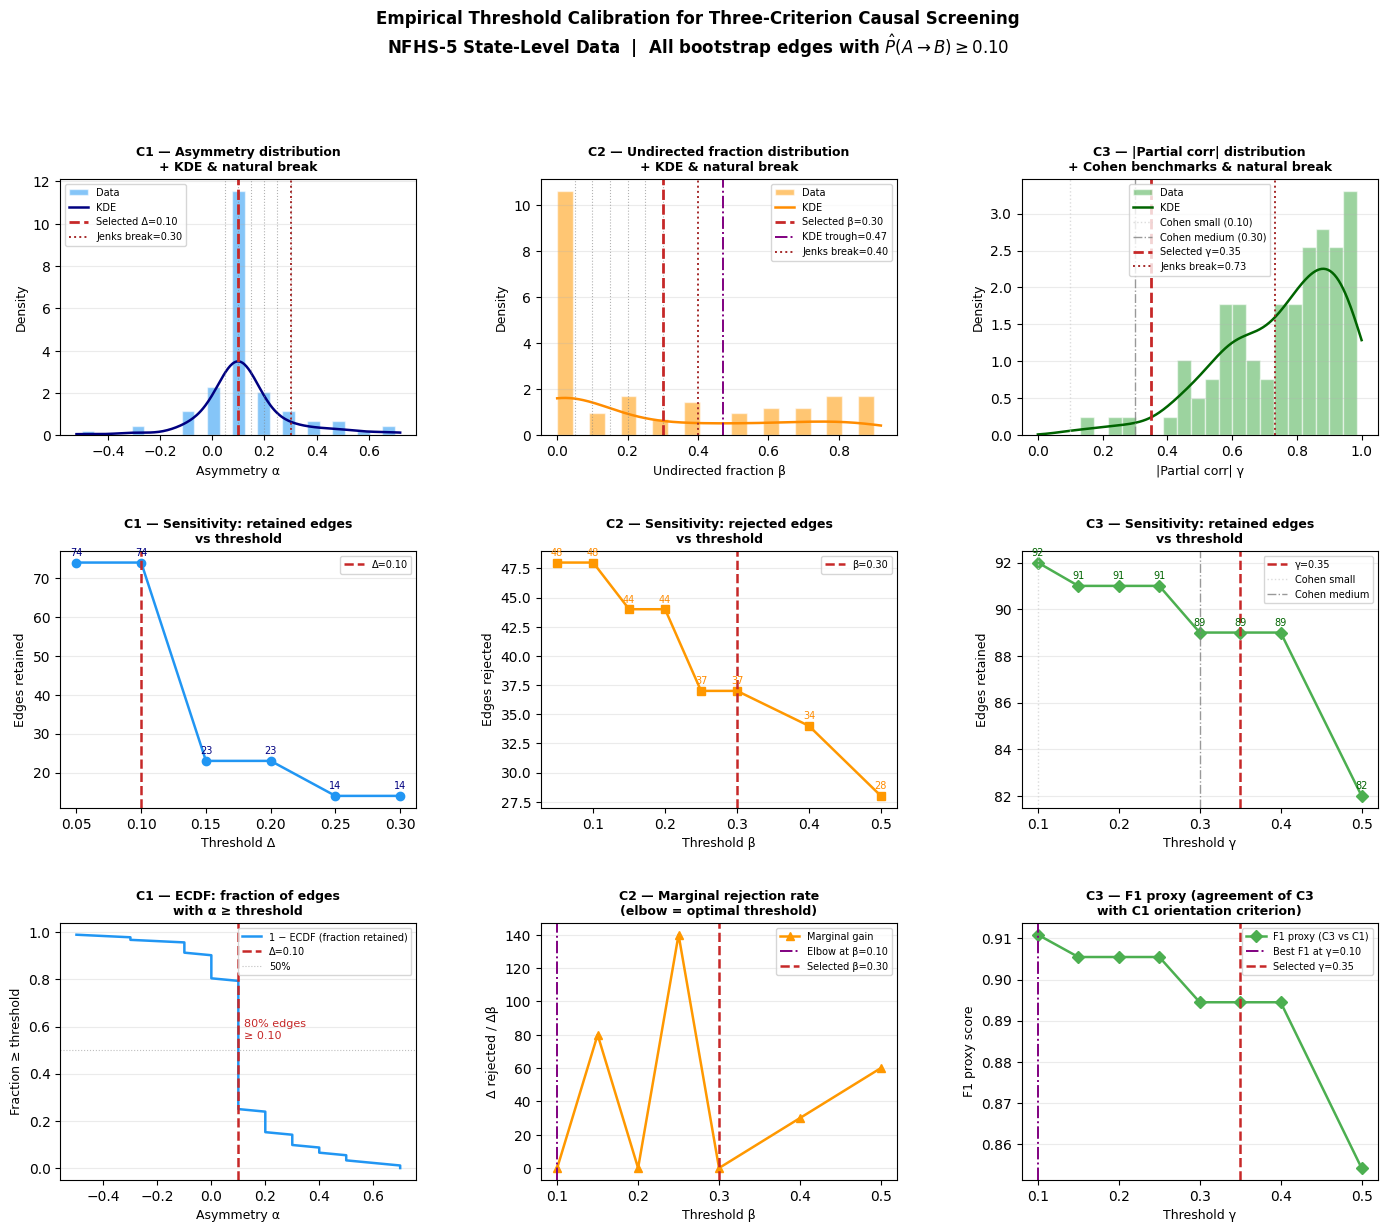
\includegraphics[width=1.05\textwidth]{threshold_calibration_9panel.png}
\caption{Empirical calibration of the three screening criteria:
  directional asymmetry ($\Delta$), undirected-edge fraction ($\beta$), and
  partial-correlation residual magnitude ($|\rho|$). Vertical dashed lines
  indicate the selected thresholds.}
\label{fig:threshold_calibration}
\end{figure}

\paragraph{Criterion 1: Directional asymmetry ($\Delta$).}
The asymmetry distribution is strongly concentrated near zero. The selected
threshold $\Delta=0.10$ coincides with the bootstrap confidence floor and retains
approximately 80\% of candidate edges, whereas larger thresholds lead to abrupt
reductions without corresponding increase in directional certainty.

\paragraph{Criterion 2: Undirected-edge fraction ($\beta$).}
The distribution of $\beta$ exhibits a clear separation between low-ambiguity and
highly ambiguous edges. The KDE trough ($\beta\approx0.47$) and Jenks break
($\beta\approx0.40$) indicate a transition region beyond which orientations become
unstable. Selected: $\beta<0.30$.

\paragraph{Criterion 3: Partial-correlation residual ($|\rho|$).}
The F1-proxy remains nearly constant for thresholds between 0.10 and 0.40, while
edge retention begins to decline more rapidly beyond $\gamma=0.35$.
Selected: $|\rho|\ge0.35$.

\chapter{Candidate Pathway Pool (14 Pathways)}
\label{app:pathway_selection}

\begin{table}[H]
\centering
\caption{14 candidate pathways and selection outcome. ``Pooled'' = consistent
  across $\ge3/4$ estimators in pooled analysis. ``Selected'' = also achieves
  stratification consistency.}
\label{tab:candidate_pathways}
\renewcommand{\arraystretch}{1.2}
\begin{tabular}{clcc}
\toprule
\textbf{\#} & \textbf{Pathway} & \textbf{Pooled} & \textbf{Selected} \\
\midrule
1  & Solid Food \& BF $\to$ Diarrhoea (ORS)            & Partial & No \\
2  & FP(Any) $\to$ BCG Vaccination                     & \checkmark & No \\
3  & Pregnant Anaemia $\to$ Excl.\ Breastfeeding        & \checkmark & No \\
4  & FP(Any) $\to$ Unmet Need for Spacing               & \checkmark & \textbf{Yes} \\
5  & FP(Any) $\to$ Neonatal Tetanus Protection          & \checkmark & \textbf{Yes} \\
6  & Physical Violence $\to$ HH Decision Participation  & \checkmark & No \\
7  & ANC (First Trimester) $\to$ Home Births (Facility) & \checkmark & \textbf{Yes} \\
8  & Postnatal Care $\to$ Vitamin A Dose                & Partial & No \\
9  & Women Elevated BP $\to$ C-Section (Public)         & \checkmark & \textbf{Yes} \\
10 & Women Tobacco $\to$ Children Overweight            & Partial & No \\
11 & Women Literacy $\to$ Mobile Phone Ownership        & \checkmark & \textbf{Yes} \\
12 & FP(Any) $\to$ Diarrhoea (Taken to Facility)        & Partial & No \\
13 & Men Internet Use $\to$ Men Literacy                & \checkmark & \textbf{Yes} \\
14 & Pregnant Anaemia $\to$ Child Anaemia (6--59m)      & Partial & No \\
\bottomrule
\end{tabular}
\end{table}

\chapter{Exploratory Correlation Analysis}
\label{app:corr}

\section*{Indicator Distributions}

\begin{figure}[H]
\centering
\begin{subfigure}{0.45\textwidth}
  \includegraphics[width=\linewidth]{nmr.png}
  \caption{Approximately zero-skewed (NMR)}
\end{subfigure}
\hfill
\begin{subfigure}{0.45\textwidth}
  \includegraphics[width=\linewidth]{institutional_births.png}
  \caption{Left-skewed (Institutional births)}
\end{subfigure}
\vspace{6pt}
\begin{subfigure}{0.45\textwidth}
  \includegraphics[width=\linewidth]{family_planing.png}
  \caption{Left-skewed (Family planning)}
\end{subfigure}
\hfill
\begin{subfigure}{0.45\textwidth}
  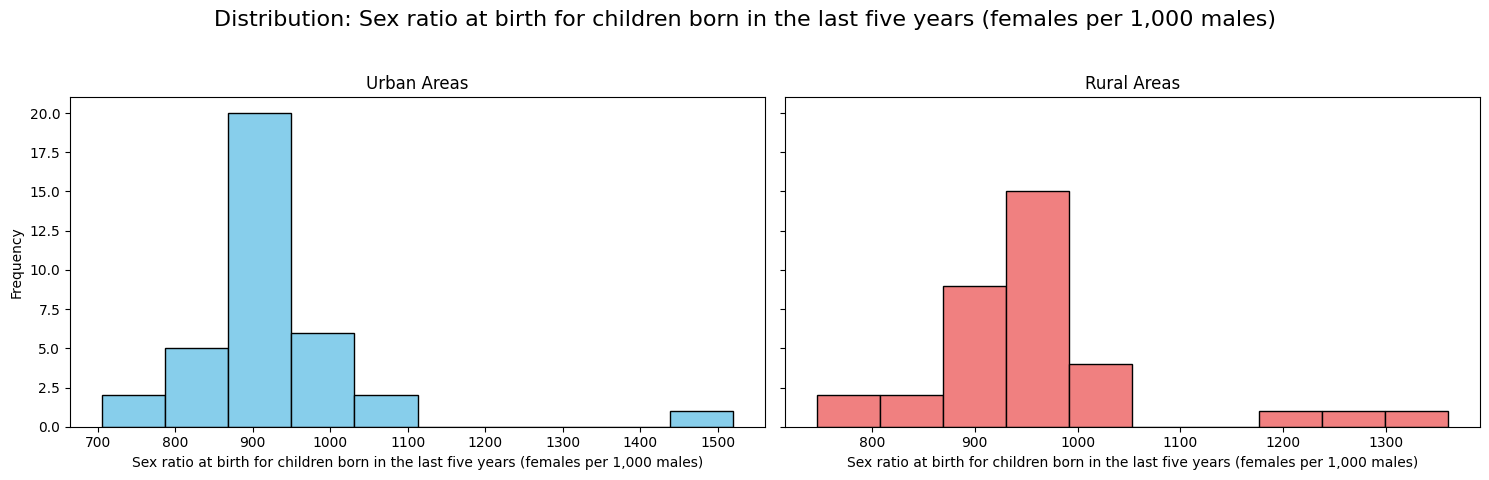
\includegraphics[width=\linewidth]{sex_ratio_at_birth.png}
  \caption{Right-skewed (Sex ratio at birth)}
\end{subfigure}
\caption{Indicator-level distribution diagnostics.}
\label{fig:distribution_diagnostics}
\end{figure}

\section*{Correlation Rank Plots}

\begin{figure}[H]
\centering
\begin{subfigure}{0.48\textwidth}
  \includegraphics[width=\linewidth]{line_plot_corr_1.png}
  \caption{Overall: right-skewed, ${\sim}10$ pairs $|r|>0.70$.}
\end{subfigure}
\hfill
\begin{subfigure}{0.48\textwidth}
  \includegraphics[width=\linewidth]{plots/line_plot_area_corr_1.png}
  \caption{Area-stratified: rural stronger than urban.}
\end{subfigure}
\vspace{6pt}
\begin{subfigure}{0.48\textwidth}
  \includegraphics[width=\linewidth]{plots/line_plot_sgdp_corr_1.png}
  \caption{Income-stratified: nearly identical decay.}
\end{subfigure}
\hfill
\begin{subfigure}{0.48\textwidth}
  \includegraphics[width=\linewidth]{plots/line_plot_partial_corr.png}
  \caption{Partial vs.\ stratified: partial curve lies above.}
\end{subfigure}
\caption{Correlation rank plots across four stratifications.}
\label{fig:rank_plots}
\end{figure}

\chapter{Mediation Analysis}
\label{app:mediation}

OLS models and mediation structural equations confirm that per-capita GSDP is a
weak direct confounder (proportion mediated $=-2.14\%$), while mediation through
women's literacy is significant.
This motivated adopting women's literacy alongside GSDP as the joint confounder
set $\bZ$.

\begin{figure}[H]
\centering
\begin{subfigure}{0.28\textwidth}
  \includegraphics[width=\linewidth]{proposed_dag.png}
  \caption{Proposed causal DAG}
\end{subfigure}
\hfill
\begin{subfigure}{0.65\textwidth}
  \includegraphics[width=\linewidth]{OLS_results.png}
  \caption{OLS regression results}
\end{subfigure}
\caption{Proposed DAG and OLS regression summary for mediation analysis.}
\label{fig:mediation}
\end{figure}

\chapter{Clustering Figures}
\label{app:clustering_figs}

\begin{figure}[H]
\centering
\includegraphics[width=0.95\textwidth]{heirarchical_cluster_1.png}
\caption{Hierarchical clustering dendrogram ($k=32$ cut shown).}
\label{fig:dendrogram}
\end{figure}

\begin{figure}[H]
\centering
\includegraphics[width=0.95\textwidth]{plots/mod_vs_res.png}
\caption{Parameter sweep: Louvain/Leiden modularity and $k$ vs.\ resolution (top);
  silhouette vs.\ resolution (bottom-left); Spectral silhouette vs.\ $n$ clusters
  (bottom-right).}
\label{fig:cluster_param_sweep}
\end{figure}

\begin{figure}[H]
\centering
\begin{subfigure}{0.98\textwidth}
  \includegraphics[width=\linewidth]{louvain.png}
  \caption{Louvain ($\gamma=3.0$)}
\end{subfigure}
\hfill
\begin{subfigure}{0.98\textwidth}
  \includegraphics[width=\linewidth]{leiden.png}
  \caption{Leiden ($\gamma=3.0$)}
\end{subfigure}
\vspace{6pt}
\begin{subfigure}{0.98\textwidth}
  \centering
  \includegraphics[width=\linewidth]{spectral_clustering.png}
  \caption{Spectral ($k=28$)}
\end{subfigure}
\caption{Graph-based clustering solutions.}
\label{fig:graph_clustering}
\end{figure}

\chapter{Causal Discovery Figures}
\label{app:causal_figs}

\begin{figure}[H]
\centering
\begin{subfigure}{0.48\textwidth}
  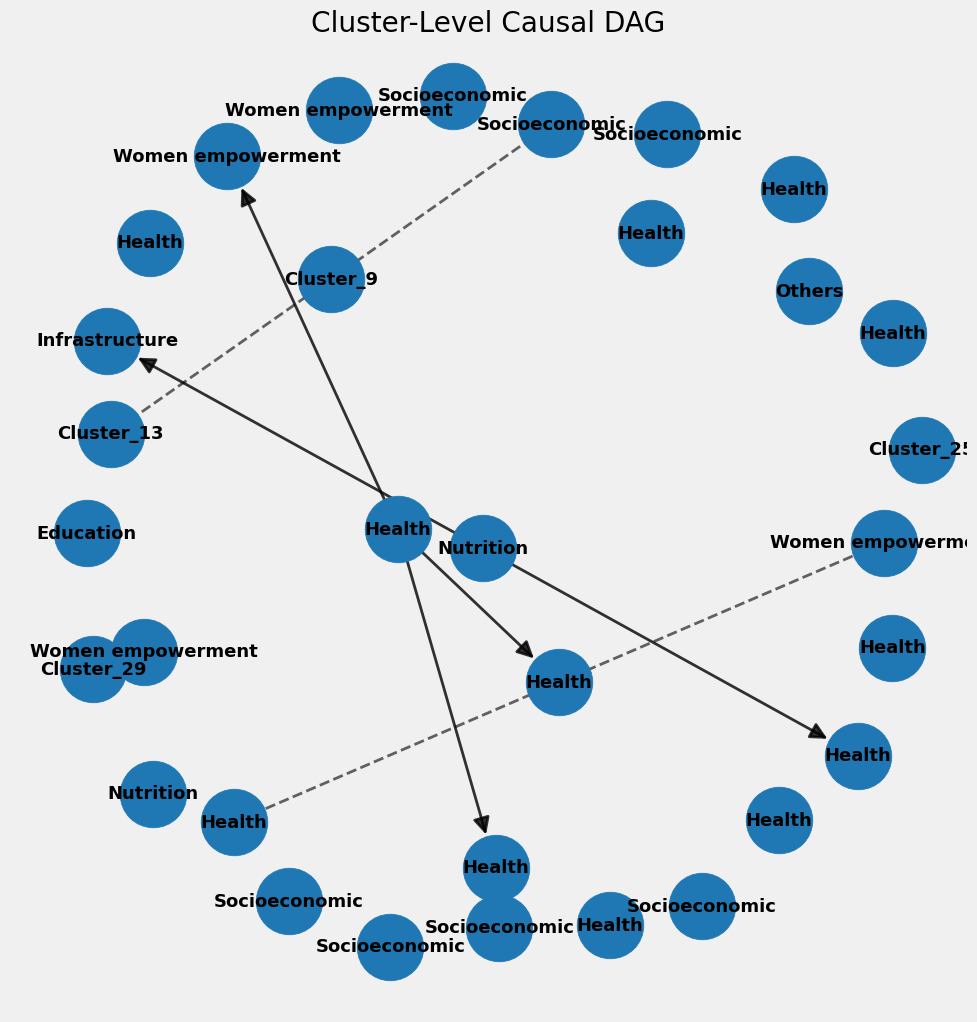
\includegraphics[width=\linewidth]{cluster_level_causal_dag_3.png}
  \caption{Inter-cluster DAG}
\end{subfigure}
\hfill
\begin{subfigure}{0.48\textwidth}
  \includegraphics[width=\linewidth]{intra_cluster_graph.png}
  \caption{Intra-cluster DAG}
\end{subfigure}
\caption{Two-level causal structure: macro (inter-cluster) and micro
  (intra-cluster) DAGs from PC discovery.}
\label{fig:dag_comparison}
\end{figure}

\begin{figure}[H]
\centering
\includegraphics[width=0.95\textwidth]{plots/boostrap_thres_analysis.png}
\caption{Bootstrap threshold sensitivity analysis (100 resamples).
  Left: retained directed edges; centre: undirected-edge fraction; right:
  isolated nodes. Knee at $\tau=0.10$ (red dashed).}
\label{fig:boot_threshold}
\end{figure}

\begin{figure}[H]
\centering

\includegraphics[width=0.95\textwidth]{plots/cluster_1_edge_confidence_1.png}
\caption{Intra-cluster DAG for Cluster~1 with bootstrap edge confidence scores.}
\label{fig:cluster1_dag}
\end{figure}

\begin{figure}[H]
\centering
\includegraphics[width=0.95\textwidth]{plots/distribution_of_edge_conf.png}
\caption{Distribution of bootstrap confidence values for Cluster~1 directed edges.}
\label{fig:boot_conf_dist}
\end{figure}

\chapter{Full ATE Tables and Heatmaps}
\label{app:ate_tables}

\begin{table}[H]
\centering
\caption{Pooled ATE estimates (percentage points) for six causal pathways across
  four estimators ($n=24$--28 states). A checkmark denotes $\ge3/4$ estimators
  agree on sign.}
\label{tab:ate_comparison}
\renewcommand{\arraystretch}{1.3}
\setlength{\tabcolsep}{4pt}
\begin{tabular}{p{4.5cm}cccccc}
\toprule
\textbf{Pathway} & \textbf{IPW} & \textbf{DR} & \textbf{T} & \textbf{X} &
\textbf{Median} & \textbf{Cons.} \\
\midrule
FP $\to$ Unmet Spacing
  & $-2.81$ & $-3.85$ & $-3.04$ & $-3.41$ & $-3.22$ & \checkmark \\
FP $\to$ Neonatal Tetanus
  & $+5.90$ & $+7.53$ & $+5.21$ & $+4.90$ & $+5.55$ & \checkmark \\
ANC $\to$ Home Births
  & $+3.30$ & $+1.04$ & $+2.17$ & $+1.22$ & $+1.70$ & \checkmark \\
Elevated BP $\to$ C-Section
  & $+9.99$ & $+13.79$ & $+9.42$ & $+8.64$ & $+9.71$ & \checkmark \\
Literacy $\to$ Mobile Phone
  & $+17.15$ & $+19.81$ & $+12.73$ & $+5.84$ & $+14.94$ & \checkmark \\
Men Internet $\to$ Men Literacy
  & $+5.01$ & $+4.88$ & $+4.06$ & $+3.44$ & $+4.47$ & \checkmark \\
\bottomrule
\end{tabular}
\end{table}

\begin{table}[H]
\centering
\caption{95\% confidence intervals for pooled ATE estimates.}
\label{tab:ate_ci}
\renewcommand{\arraystretch}{1.3}
\setlength{\tabcolsep}{4pt}
\begin{tabular}{p{4cm}cccc}
\toprule
\textbf{Pathway} & \textbf{IPW} & \textbf{DR Learner} &
\textbf{T-Learner} & \textbf{X-Learner} \\
\midrule
FP $\to$ Spacing
  & $[-4.45,\,-1.17]$ & $[-6.50,\,-1.20]$ & $[-4.80,\,-1.29]$ & $[-5.36,\,-1.45]$ \\
FP $\to$ Neonatal Tetanus
  & $[3.26,\,8.54]$ & $[3.18,\,11.89]$ & $[1.52,\,8.89]$ & $[0.79,\,9.02]$ \\
ANC $\to$ Home Births
  & $[0.11,\,6.49]$ & $[-3.76,\,5.84]$ & $[-1.16,\,5.50]$ & $[-2.88,\,5.33]$ \\
Elevated BP $\to$ C-Section
  & $[5.41,\,14.57]$ & $[4.88,\,22.71]$ & $[3.34,\,15.51]$ & $[0.30,\,16.98]$ \\
Literacy $\to$ Mobile Phone
  & $[8.19,\,26.12]$ & $[7.61,\,32.01]$ & $[3.96,\,21.51]$ & $[-5.40,\,17.07]$ \\
Men Internet $\to$ Literacy
  & $[2.37,\,7.64]$ & $[1.50,\,8.26]$ & $[1.53,\,6.59]$ & $[-0.32,\,7.20]$ \\
\bottomrule
\end{tabular}
\end{table}

\begin{figure}[H]
\centering

\includegraphics[width=0.95\textwidth]{plots/causal_ate_heatmap_14paths.png}
\caption{ATE heatmap (pathway $\times$ estimator). Blue: negative; red: positive.
  Consistent direction across all four estimators visible for all six pathways.}
\label{fig:ate_heatmap}
\end{figure}

\begin{table}[H]
\centering
\caption{Area-stratified ATE estimates (percentage points).
  \textit{Consistent}: $\ge3/4$ estimators agree on sign.}
\label{tab:area_ate}
\renewcommand{\arraystretch}{1.25}
\setlength{\tabcolsep}{3pt}
\small
\begin{tabular}{llrrrrrr}
\toprule
\textbf{Pathway} & \textbf{Area} &
\textbf{IPW} & \textbf{DR} & \textbf{T-Lrn} & \textbf{X-Lrn} &
\textbf{Median} & \textbf{Cons.} \\
\midrule
\multirow{2}{*}{FP $\to$ Spacing}
  & Rural & $-2.90$ & $-3.50$ & $-3.13$ & $-3.23$ & $-3.18$ & \checkmark \\
  & Urban & $-3.06$ & $-3.62$ & $-2.76$ & $-3.06$ & $-3.06$ & \checkmark \\[2pt]
\multirow{2}{*}{FP $\to$ Neonatal Tetanus}
  & Rural & $+4.84$ & $+8.34$ & $+6.27$ & $+6.53$ & $+6.40$ & \checkmark \\
  & Urban & $+3.03$ & $+3.40$ & $+4.66$ & $+6.16$ & $+4.03$ & \checkmark \\[2pt]
\multirow{2}{*}{ANC $\to$ Home Births}
  & Rural & $+2.67$ & $+2.96$ & $+1.52$ & $+3.37$ & $+2.81$ & \checkmark \\
  & Urban & $-1.77$ & $-2.14$ & $-1.53$ & $+0.43$ & $-1.65$ & Partial \\[2pt]
\multirow{2}{*}{Elevated BP $\to$ C-Section}
  & Rural & $+9.49$ & $+10.36$ & $+6.07$ & $+2.92$ & $+7.78$ & \checkmark \\
  & Urban & $+11.97$ & $+17.34$ & $+12.27$ & $+11.49$ & $+12.12$ & \checkmark \\[2pt]
\multirow{2}{*}{Literacy $\to$ Mobile Phone}
  & Rural & $+18.74$ & $+21.18$ & $+18.85$ & $+13.84$ & $+18.80$ & \checkmark \\
  & Urban & $+10.68$ & $+10.62$ & $+10.07$ & $+8.58$ & $+10.34$ & \checkmark \\[2pt]
\multirow{2}{*}{Men Internet $\to$ Literacy}
  & Rural & $+6.40$ & $+6.73$ & $+5.09$ & $+5.01$ & $+5.74$ & \checkmark \\
  & Urban & $+2.64$ & $+3.97$ & $+2.18$ & $+2.10$ & $+2.41$ & \checkmark \\
\bottomrule
\end{tabular}
\end{table}

\begin{table}[H]
\centering
\caption{Income-stratified ATE estimates (percentage points).
  GSDP: Low ($\lesssim$\,Rs.\,90k), Moderate, High ($\gtrsim$\,Rs.\,180k).}
\label{tab:income_ate}
\renewcommand{\arraystretch}{1.25}
\setlength{\tabcolsep}{3pt}
\small
\begin{tabular}{llrrrrrr}
\toprule
\textbf{Pathway} & \textbf{GSDP} &
\textbf{IPW} & \textbf{DR} & \textbf{T-Lrn} & \textbf{X-Lrn} &
\textbf{Median} & \textbf{Cons.} \\
\midrule
\multirow{3}{*}{FP $\to$ Spacing}
  & Low      & $-2.85$ & $-0.50$ & $-5.55$ & $-5.39$ & $-4.12$ & \checkmark \\
  & Moderate & $-3.53$ & $-3.37$ & $-3.29$ & $-2.59$ & $-3.33$ & \checkmark \\
  & High     & $-0.88$ & $-1.05$ & $-0.70$ & $-0.46$ & $-0.79$ & \checkmark \\[2pt]
\multirow{3}{*}{FP $\to$ Neonatal TT}
  & Low      & $+3.20$ & $+1.20$ & $+4.53$ & $+4.45$ & $+3.82$ & \checkmark \\
  & Moderate & $+12.26$ & $+14.08$ & $+11.83$ & $+12.67$ & $+12.46$ & \checkmark \\
  & High     & $-0.93$ & $+0.30$ & $-0.65$ & $-0.84$ & $-0.74$ & Partial \\[2pt]
\multirow{3}{*}{ANC $\to$ Home Births}
  & Low      & $+0.42$ & $+2.60$ & $+0.72$ & $+0.74$ & $+0.73$ & \checkmark \\
  & Moderate & $+2.74$ & $+9.37$ & $+4.88$ & $+5.34$ & $+5.11$ & \checkmark \\
  & High     & $-2.51$ & $-11.88$ & $-3.14$ & --- & $-3.14$ & \checkmark \\[2pt]
\multirow{3}{*}{BP $\to$ C-Section}
  & Low      & $+9.89$ & $+22.92$ & $+5.88$ & $+7.25$ & $+8.57$ & \checkmark \\
  & Moderate & $+10.94$ & $+13.55$ & $+11.01$ & $+10.98$ & $+10.99$ & \checkmark \\
  & High     & $+15.77$ & $+14.37$ & $+10.47$ & $+8.85$ & $+12.42$ & \checkmark \\[2pt]
\multirow{3}{*}{Literacy $\to$ Mobile}
  & Low      & $+13.71$ & $+28.52$ & $+12.80$ & $+13.90$ & $+13.81$ & \checkmark \\
  & Moderate & $+20.18$ & $+13.08$ & $+16.54$ & $+15.97$ & $+16.26$ & \checkmark \\
  & High     & $+27.15$ & $+27.92$ & $+26.41$ & $+23.04$ & $+26.78$ & \checkmark \\[2pt]
\multirow{3}{*}{Internet $\to$ Literacy}
  & Low      & $+4.65$ & $+15.98$ & $+4.54$ & $+4.84$ & $+4.75$ & \checkmark \\
  & Moderate & $+3.76$ & $+8.12$ & $+7.13$ & $+8.87$ & $+7.63$ & \checkmark \\
  & High     & $+4.46$ & $+2.01$ & $+4.87$ & $+4.51$ & $+4.49$ & \checkmark \\
\bottomrule
\end{tabular}
\end{table}

\begin{figure}[H]
\centering

\includegraphics[width=0.88\textwidth]{plots/causal_income_ate_heatmap_14paths.png}
\caption{Median ATE heatmap by pathway and income stratum.
  Blue: negative; red: positive.}
\label{fig:income_heatmap}
\end{figure}

\end{appendices}

\end{document}